\documentclass[preprint,12pt]{elsarticle}
\biboptions{sort&compress}
\usepackage{amsmath}
\usepackage{amsfonts}
\usepackage{amssymb}
\usepackage{graphicx}
\usepackage{hyperref}
\usepackage{tabls}
\usepackage{multirow}
\usepackage{cleveref}
\usepackage{verbatim}

\usepackage{pgfplots}
\usetikzlibrary{plotmarks}
\usepackage{tikz}
\usetikzlibrary{shapes,arrows}
\newcommand*{\h}{\hspace{5pt}}% for indentation
\newcommand*{\hh}{\h\h}% double indentation

\usepackage{framed} % Framing content
\usepackage{multicol} % Multiple columns environment
\usepackage{nomencl} % Nomenclature package
\RequirePackage{ifthen}
\renewcommand{\nomgroup}[1]{%
\ifthenelse{\equal{#1}{P}}{\item[\textbf{Superscripts}]}{
\ifthenelse{\equal{#1}{G}}{\item[\textbf{Greek Symbols}]}{
\ifthenelse{\equal{#1}{S}}{\item[\textbf{Subscripts}]}{}}}}

\newcommand{\nomunit}[1]{%
\renewcommand{\nomentryend}{\hspace*{\fill}#1}}
\newcommand{\bv}[1]{\boldsymbol #1}  % change this to change how math vectors are handled

%\usepackage{breqn}

%\special{papersize=8.5in,11in}

\journal{International Journal of Heat and Mass Transfer}


\pdfinfo{%
  /Title(Optimization of an Inverse Convection Solution Strategy)
  /Author   (Yogesh Jaluria)
    /Author   (Joseph R VanderVeer)
  /Creator  (Joseph R VanderVeer)
  /Subject  (Inverse Convection Problems)
}

\begin{document}

\begin{frontmatter}
\title{Optimization of an Inverse Convection Solution Strategy}

\author{Joseph R VanderVeer}
\author{Yogesh Jaluria\corref{cor}}
\ead{jaluria@soemail.rutgers.edu}

\address{Department of Mechanical and Aerospace Engineering: Rutgers University, 98 Brett Rd, Piscataway NJ, 08854}
\cortext[cor]{Corresponding Author}



\begin{abstract}



\end{abstract}
\begin{keyword}
Inverse Problems \sep Computational Heat Transfer \sep Convection
\end{keyword}
\end{frontmatter}

\crefname{equation}{equation}{equations}
\crefname{figure}{figure}{figures}
\crefname{table}{table}{tables}

\newlength\figureheight 
\newlength\figurewidth 
	
	
	
	
\makenomenclature
\setlength{\nomitemsep}{-\parskip} % Baseline skip between items
\renewcommand*\nompreamble{\begin{multicols}{2}}
\renewcommand*\nompostamble{\end{multicols}}
\nomenclature[A]{$T$}{temperature}
\nomenclature[G]{$\bv{\Delta}$}{relative difference between the first sampled point and other sampled points}
\nomenclature[A]{$\bv{r}$}{vector location of sampled points}
\nomenclature[A]{$F$}{minimization function}
\nomenclature[A]{$n$}{number of sample locations}
\nomenclature[G]{$\bv{\delta}$}{vector distance between the actual sampled location and the current test location}
\nomenclature[G]{$\varepsilon$}{error associated with the inverse convection method at a location with given sampled data}
\nomenclature[A]{$d$}{number of simulations}
\nomenclature[A]{$a$}{number of sample locations used in the predictor stage}
\nomenclature[A]{$U$}{free stream velocity}
\nomenclature[A]{$x,y$}{coordinates}
\nomenclature[G]{$\phi$}{normalized temperature $\phi = \frac{T-T_{\infty}}{T_S-T_{\infty}}$}
\nomenclature[A]{$X,Y$}{normalized coordinates}
\nomenclature[S]{$i, j,k$}{index}
\nomenclature[S]{$A,B$}{data set A,B}
\nomenclature[S]{$P$}{predicted}
\nomenclature[S]{$mod$}{modified}
\nomenclature[S]{$\infty$}{free stream}
\nomenclature[P]{$\ast$}{predictor stage, alternative heat flux eqn.}
\nomenclature[S]{$S$}{source}
\nomenclature[A]{$b,m$}{model parameters}
\nomenclature[S]{$0,1,2$}{sample point indexes}
\nomenclature[S]{$O$}{optimized}
\nomenclature[G]{$\rho$}{density}
\nomenclature[A]{$t$}{time}
\nomenclature[A]{$P$}{pressure}
\nomenclature[A]{$E$}{thermal energy}
\nomenclature[G]{$\mu_{t}$}{eddy viscosity}
\nomenclature[A]{$P_{rt}$}{turbulent Prandtl number}
\nomenclature[A]{$k,\epsilon$}{turbulence kinetic energy, dissipation rate}
\nomenclature[A]{$C_1,C_2,C_{1\epsilon},C_{\mu},\sigma_k,\sigma_{\epsilon}$}{$k-\epsilon$ model coefficients}
\nomenclature[A]{$l, I$}{turbulence length scale and intensity}
\nomenclature[G]{$\lambda$}{thermal conductivity}
\nomenclature[G]{$\mu$}{dynamic viscosity}

%\nomenclature[A]{ }{ }

\begin{table*}[!t]
  \begin{framed}
    \printnomenclature
  \end{framed}
\end{table*}




\section{Introduction}
Thermal-fluid systems often create situations where the engineering problem is an inverse heat transfer problem.  These problems often have limited physical access, very limited to no boundary condition knowledge, and/or limited domain knowledge.

For example, the temperature distribution of an optical fiber drawing furnace is difficult to measure directly due to shape, inaccessibility, and high temperatures.  The center of the furnace is easily accessible and this directly leads to an inverse heat transfer problem.  \Citet{issa} \cite{issa} developed a regularization technique utilizing the centerline temperature from which the wall temperature may be obtained.

Another example, is the inverse plume in a crossflow problem.  The problem entails solving for the plume boundary conditions utilizing limited domain knowledge.  A novel predictor-corrector method was developed by \citet{ijhmt1} \cite{ijhmt1} to solve such a problem.  


The present work is the logical progression of the inverse plume in a crossflow problem, the inverse jet in a crossflow problem.  The inverse jet in a crossflow problem has many more practical applications and ...





\section{Experimental System}
The experiment consists of a wind tunnel with a surface level jet located within the test section.  The jet uses compressed air passed through flow straighteners to achieve a velocity of $U_S$ and is heated to temperature $T_S$.  The jet is subjected to a perpendicular crossflow of velocity $U_{\infty}$.  \Cref{fig:diagramjet} is a diagram of the wind tunnel and jet, dimensions are in millimeters.

\begin{figure}[!tbp]
\begin{center}
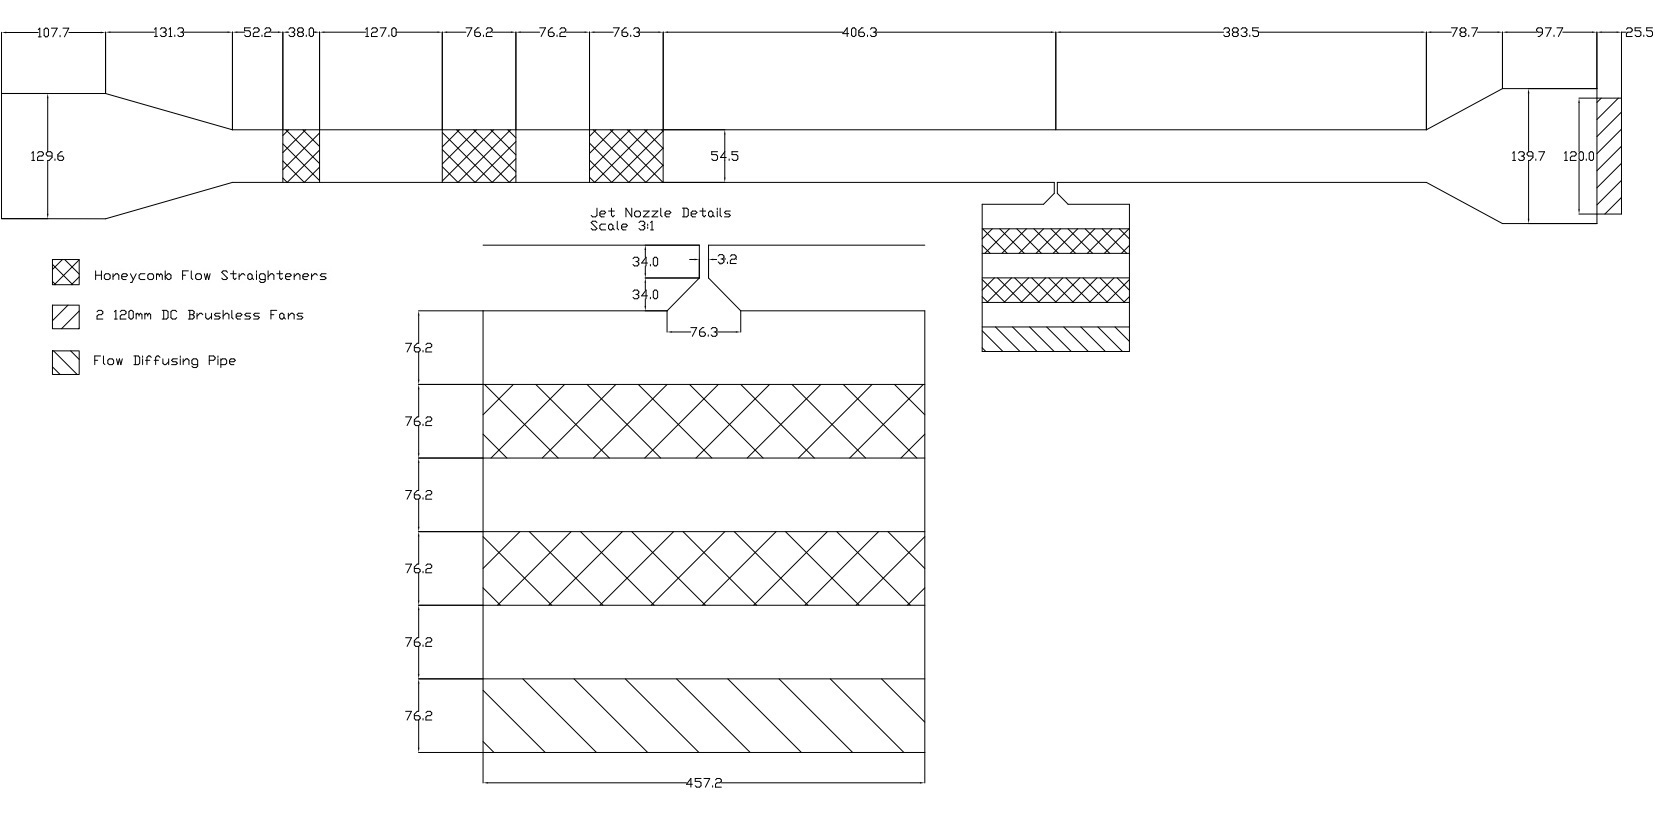
\includegraphics[scale=.30]{windtunneljet.jpg}
\caption{Schematics of the wind tunnel and jet}
\label{fig:diagramjet}
\end{center}
\end{figure}

The wind tunnel test section dimensions are $54.5\times305\times 254\,mm$.  The maximum velocity of the wind tunnel is $5.0\,m/s$.  The jet is heated by electric cartridge heaters (Omega AHP-7561) with a maximum temperature of $425\,K$ due to material limitations of the wind tunnel.  The X-direction is directed downstream of the wind tunnel with the zero at the center of the jet.  The Y-direction is in the direction of the jet and is zero at the surface of the wind tunnel.  Due to the large aspect ratio of the wind tunnel the flow is assumed to be two-dimensional.

The free stream velocity is determined by a Pitot-Static tube attached to a NIST traceable differential pressure sensor from Omega(PX655-0.1DI).  The pressure sensor has a full scale reading of 0.1 inches of water and is accurate to $0.05\%$ of full scale.  This results in a maximum of $3\%$ error of the calculated velocity.

The jet velocity is determined utilizing a rotameter and verified using a Pitot-Static tube attached to the same previously described pressure sensor.  This results in the same amount of error of $3\%$ for the jet velocity.

The temperature of domain is measured using a K-type thermocouple mounted to an X-Y traversing stage.  Sampled data over the course of several days indicate repeatability of the experiment to within $2\%$.

\section{Numerical Simulations}
The simulations were all performed using Ansys Fluent\cite{fluentsoftware}.  The Navier-Stokes equations were solved using a three-dimensional, steady state, realizable $k-\epsilon$ model with enhanced wall effects.  Conjugate heat transfer is modelled.  The free stream Reynolds number is of order $6\times10^3$, while the jet Reynolds number is between $10^3$ and $10^4$.  The Rayleigh number is of order $10^7$.

The governing equations are expressed below:

\begin{equation}
\centering
u_i = \overline{u_i} + u^{'}_{i}
\label{eq:veldecomp}
\end{equation}

\begin{equation}
\frac{\partial \rho }{\partial t } + \frac{\partial }{\partial x_i} \left( \rho u_i \right) = 0 
\label{eq:mass}
\end{equation}

\begin{equation}
\centering
\begin{split}
\frac{\partial }{\partial t} \left( \rho u_i \right) &+ \frac{\partial }{\partial x_j } \left( \rho u_i u_j \right) = \\
 &\frac{\partial P}{\partial x_i } + \frac{\partial }{\partial x_j } \left[ \mu \left( 2 S_{ij} - \frac{2}{3} \delta_{ij} \frac{\partial u_k }{\partial x_k } \right) - \rho \overline{u^{'}_{i} u^{'}_{j}} \right] 
\label{eq:momentum}
\end{split}
\end{equation}

\begin{equation}
\centering
\begin{split}
\frac{\partial }{\partial t } \left( \rho E \right) &+ \frac{\partial }{\partial x_i} \left[ u_i \left( \rho E + P \right) \right] = \\
 &\frac{\partial }{\partial x_i } \left[ \left( \lambda + \frac{C_p \mu_t }{P_{rt}} \right) \frac{\partial T}{\partial x_i} \right] 
\label{eq:energy}
\end{split}
\end{equation}

\begin{equation}
\centering
\begin{split}
\frac{\partial }{\partial t} \left(\rho k \right) &+ \frac{\partial }{\partial x_j} \left( \rho k u_j \right) = \\
&\frac{\partial }{\partial x_j} \left[ \left( \mu + \frac{\mu_t}{\sigma_k} \right) \frac{\partial k}{\partial x_j} \right] + \frac{\partial u_j}{\partial x_i} \left( -\rho \overline{u^{'}_{i} u^{'}_{j}} \right) \\
&- g_i \frac{\mu_t}{\rho P_{rt}} \frac{\partial \rho }{\partial x_i} + \rho \epsilon
\label{eq:k}
\end{split}
\end{equation}

\begin{equation}
\centering
\begin{split}
 \frac{\partial }{\partial t} \left(\rho \epsilon \right) &+ \frac{\partial }{\partial x_j} \left( \rho \epsilon u_j \right) = \\
 &\frac{\partial }{\partial x_j } \left[ \left( \mu + \frac{\mu_t }{\sigma_\epsilon } \right) \frac{\partial \epsilon }{\partial x_j } \right] + \rho C_1 S \epsilon - \rho C_2 \frac{\epsilon^2 }{k+\sqrt{\nu \epsilon}} \\
 &- C_{1 \epsilon} \frac{\epsilon}{k} C_{3\epsilon} g_i \frac{\mu_t}{\rho P_{rt}} \frac{\partial \rho}{\partial x_i}
\label{eq:e}
\end{split}
\end{equation}

\begin{equation}
\centering
- \rho \overline{u^{'}_{i} u^{'}_{j}} = 2\mu_t S_{ij} - \frac{2}{3} \delta_{ij} \left( \rho k + \mu_t \frac{\partial u_k}{\partial x_k} \right)
\label{eq:reynoldsstress}
\end{equation}

The constants for the turbulence model are \cite{realizable,fluent} : 
\begin{equation}
\label{eq:constants}
C_{1\epsilon} = 1.44 , C_2 = 1.9 , \sigma_k = 1.0 , \sigma_\epsilon = 1.2 , P_{rt} = 0.85 
\end{equation}
\begin{equation}
C_1 = max\left[0.43,\frac{Sk/\epsilon}{Sk/\epsilon +5} \right] , S = \sqrt{2S_{ij}S_{ji}} , C_{3\epsilon} = tanh\left(\frac{u_g}{u_p}\right)
\end{equation}
\begin{subequations}
\begin{align}
\mu_t &= \frac{\rho C_{\mu} k^2}{\epsilon} \\
C_{\mu} &= \frac{1}{A_0 + \frac{A_1 k U^*}{\epsilon}} \\
U^* &\equiv \sqrt{S_{ij} S_{ji} + \Omega_{ij} \Omega_{ji}} \\
A_0 &= 4.04 \\
A_1 &= \sqrt{6} cos \left[\frac{1}{3} cos^{-1}\left(\sqrt{6} \frac{S_{ij}S_{jk}S_{ki}}{\left(S_{ij} S_{ji} \right)^{\frac{3}{2}}} \right) \right] \\
S_{ij} &= \frac{1}{2} \left( \frac{\partial u_i}{\partial x_j} + \frac{\partial u_j}{\partial x_i} \right) \\
\Omega_{ij} &= \frac{1}{2} \left( \frac{\partial u_i}{\partial x_j} - \frac{\partial u_j}{\partial x_i} \right)
\end{align}
\end{subequations}
Where the $u_g$ and $u_p$ are the velocity component parallel and perpendicular to gravity respectively.

The inflow boundary conditions are:
\begin{subequations}
\label{eq:inflow}
\begin{align}
u&=U_\infty , v=0 , T=T_\infty , P = P_\infty , l=4 mm , I=5\%\\
k&=\frac{3}{2}\left(U_\infty I\right)^2 \\
\epsilon &=C_{\mu}^{3/4} \frac{k^{3/2}}{l}
\end{align}
\end{subequations}

The jet inflow boundary conditions are:
\begin{subequations}
\label{eq:inflowjet}
\begin{align}
u&=0 , v=U_S , T=T_S , P = P_\infty , l=4 mm , I=5\%\\
k&=\frac{3}{2}\left(U_\infty I\right)^2 \\
\epsilon &=C_{\mu}^{3/4} \frac{k^{3/2}}{l}
\end{align}
\end{subequations}

The upper boundary was taken to be symmetric to reduce the possibility of errors by the experimentally accurate no-slip condition.  The upper boundary is very far from the jet and therefore should have negligible effect on the numerical result.  The bottom of the wind tunnel is made up of $12\, mm$ thick acrylic, while the test section is $25.4\,mm$ thick acrylic.  The external boundary conditions are iso-thermal with a temperature of $T_{\infty}$.  The test section external temperature is iso-thermal of $\frac{1}{2}\left(T_S+T_{\infty}\right)$.  The outflow boundary is a simple pressure outflow of $P_{\infty}$.

\subsection{Simulation Validation}
A simulation validation study was performed to verify the results of the simulations.  Typical verification was performed including flow model, grid independence, iterative convergence, and lastly comparison with experimental results.  The conditions of the simulation validation are shown in \cref{tab:VTjet}.

\begin{table}[!t!b!p]
\begin{center}
\begin{tabular}{ c c }
\hline
Parameter    & Value \\ \hline
$U_{\infty} \, (m/s)$ & $2.0\pm0.02$ \\
$U_S \, (m/s)$ & $2.0\pm0.2$ \\
$T_{\infty} \, (K) $ & $305\pm0.5$ \\
$P_{\infty} \, (kPa) $ & $101.3\pm0.01$ \\
$T_{S} \, (K) $ & $350\pm2.0$ \\ \hline
\end{tabular}
\caption{Validation test conditions}
\label{tab:VTjet}
\end{center}
\end{table}

The results from Spalart-Allmaras, $k-\epsilon$, and $k-\omega$ were compared and the three models have a similar trend.  SA tends to be a bit off, but this is expected due to issues with this type of problem\cite{fluent}.  All of the values were normalized utilizing the following equations, where $D$ is the width of the jet.  \Cref{fig:jetmodel15mm} shows a comparison of the flow models at $X=4.75$.
\begin{align}
\phi &= \frac{T-T_{\infty}}{T_S-T_{\infty}} \\
X &= \frac{x}{D} \\
Y &= \frac{y}{D} \\
V &= \frac{U}{U_\infty}  \\
V_S &= \frac{U_S}{U_{\infty}}
\end{align}
\end{subequations}
\begin{figure}[!tbp]
	\centering
  \setlength\figureheight{5cm} 
	\setlength\figurewidth{5cm}
	% This file was created by matlab2tikz v0.2.1.
% Copyright (c) 2008--2012, Nico Schlömer <nico.schloemer@gmail.com>
% All rights reserved.
% 
% The latest updates can be retrieved from
%   http://www.mathworks.com/matlabcentral/fileexchange/22022-matlab2tikz
% where you can also make suggestions and rate matlab2tikz.
% 
% 
% 
\begin{tikzpicture}

\begin{axis}[%
view={0}{90},
width=\figurewidth,
height=\figureheight,
scale only axis,
xmin=0, xmax=0.8,
xlabel={Normalized Temperature},
ymin=0, ymax=5,
ylabel={Normalized Distance Above Surface (Y-axis)},
axis lines=left,
legend style={nodes=right}]
\addplot [
color=black,
dashed,
line width = 1.5pt
]
coordinates{
 (0.598022194358906,0)(0.719633644440864,0.31496062992126)(0.773342793297479,0.62992125984252)(0.787137560078285,0.94488188976378)(0.786982506712231,1.25984251968504)(0.767485577679692,1.5748031496063)(0.716462238981407,1.88976377952756)(0.621973697060202,2.20472440944882)(0.480706343310905,2.51968503937008)(0.311097850416844,2.83464566929134)(0.160803897231797,3.1496062992126)(0.0691451576006809,3.46456692913386)(0.0249505232734139,3.77952755905512)(0.00763753550304175,4.09448818897638)(0.00197928210192474,4.40944881889764)(0.000359340398558418,4.7244094488189) 
};

\addlegendentry{SA};

\addplot [
color=black,
solid,
line width = 1.5pt
]
coordinates{
 (0.475508101325801,0)(0.550052890287577,0.31496062992126)(0.55412002610574,0.62992125984252)(0.531443362113594,0.94488188976378)(0.496125463740959,1.25984251968504)(0.450496289862748,1.5748031496063)(0.3934550283275,1.88976377952756)(0.328670791774968,2.20472440944882)(0.262813124212552,2.51968503937008)(0.199826985242342,2.83464566929134)(0.143142443504267,3.1496062992126)(0.0963463996907779,3.46456692913386)(0.0601829585553529,3.77952755905512)(0.0358385592290458,4.09448818897638)(0.0192371842163784,4.40944881889764)(0.00922113373690982,4.7244094488189) 
};

\addlegendentry{k-e};

\addplot [
color=black,
dotted,
line width = 1.5pt
]
coordinates{
 (0.623553431329684,0)(0.72099881236359,0.31496062992126)(0.751725742420293,0.62992125984252)(0.769701953149541,0.94488188976378)(0.779485121151673,1.25984251968504)(0.770323219262517,1.5748031496063)(0.724627008448031,1.88976377952756)(0.628332228898429,2.20472440944882)(0.472876701362613,2.51968503937008)(0.283070581920853,2.83464566929134)(0.133380285447469,3.1496062992126)(0.0586545740916514,3.46456692913386)(0.0258944594893283,3.77952755905512)(0.012059155531458,4.09448818897638)(0.0058223208773638,4.40944881889764)(0.00276500998016413,4.7244094488189) 
};

\addlegendentry{k-w};

\end{axis}
\end{tikzpicture}

	\caption{Validation of the simulation: local temperature using three flow models at $X=4.75$}
	\label{fig:jetmodel15mm}
\end{figure}

Grid independence is demonstrated by testing the temperature at a few locations with various grid sizes and geometries, as shown in \cref{tab:gridjet}.  Very little variation in simulated temperature over such a wide variety of cell counts shows that the result is most likely grid independent.  The grid employed is an unstructured hexagonal mesh with refinement located near the jet and down stream of the jet.
\begin{table}[!t!b!p]
\begin{center}
\begin{tabular}{ c c c c c }
\hline
 Location (x,y) (mm) & 0,1 & 10,5 & 15,5& 30,10 \\ \hline \hline
 Cell Count & \\ \hline
 57660  & 337.7 & 323.3 & 321.6 & 310.1 \\ \hline
 83888  & 337.7 & 323.3 & 321.6 & 310.1 \\ \hline
 166352 & 337.7 & 323.2 & 321.5 & 310.1 \\ \hline
 366168 & 337.7 & 323.2 & 321.5 & 310.1 \\ \hline
\end{tabular}
\caption{Grid Independence Study, local static temperature (K)}
\label{tab:gridjet}
\end{center}
\end{table}

Iterative convergence is typically proven by increasing the residual requirements to very tiny amounts.  In this case, due to the extremely small elements within the jet, a residual of $10^{-8}$ was used.  \Cref{fig:jetiterate15mm} is a plot of error compared to the $10^{-8}$ residuals for several residual cases.  It can be seen that the error is progressively reducing and a residual of $10^{-6}$ should give acceptable iterative errors (experimental - numerical errors will be much larger).
\begin{figure}[!htbp]
	\centering
  \setlength\figureheight{7cm} 
	\setlength\figurewidth{7cm}
	% This file was created by matlab2tikz v0.2.1.
% Copyright (c) 2008--2012, Nico Schlömer <nico.schloemer@gmail.com>
% All rights reserved.
% 
% The latest updates can be retrieved from
%   http://www.mathworks.com/matlabcentral/fileexchange/22022-matlab2tikz
% where you can also make suggestions and rate matlab2tikz.
% 
% 
% 
\begin{tikzpicture}

\begin{semilogyaxis}[%
view={0}{90},
width=\figurewidth,
height=\figureheight,
scale only axis,
xmin=0, xmax=5,
xlabel={Normalized distance above surface (Y-axis)},
ymin=1e-07, ymax=1,
yminorticks=true,
ylabel={$\text{Error in temperature from 10}^\text{-8}\text{ residual solution}$},
legend style={at={(0.97,0.03)},anchor=south east,nodes=right}]
\addplot [
color=black,
solid,
line width = 1.5pt
]
coordinates{
 (0,0.183570039895699)(0.31496062992126,0.119677394602206)(0.62992125984252,0.0597678374185762)(0.94488188976378,0.0418913694597904)(1.25984251968504,0.0546738639469027)(1.5748031496063,0.111687747425776)(1.88976377952756,0.214670181029362)(2.20472440944882,0.305412872110992)(2.51968503937008,0.366805042231704)(2.83464566929134,0.415767406934549)(3.1496062992126,0.462479217653083)(3.46456692913386,0.482454684632103)(3.77952755905512,0.43377134001264)(4.09448818897638,0.33854894473302)(4.40944881889764,0.245785109674443)(4.7244094488189,0.194837795539684) 
};

\addlegendentry{$\text{10}^\text{-3}\text{ residual solution}$};

\addplot [
color=black,
dashed,
line width = 1.5pt
]
coordinates{
 (0,0.0151811582664436)(0.31496062992126,0.00883978518027106)(0.62992125984252,0.0633427719325255)(0.94488188976378,0.115325317676366)(1.25984251968504,0.168642968325742)(1.5748031496063,0.224728800892933)(1.88976377952756,0.282436260197301)(2.20472440944882,0.326207842677263)(2.51968503937008,0.346915060896265)(2.83464566929134,0.341730467759419)(3.1496062992126,0.304920656577735)(3.46456692913386,0.238907388975122)(3.77952755905512,0.158557517611655)(4.09448818897638,0.0877039804846618)(4.40944881889764,0.0323108499647446)(4.7244094488189,0.000135787316366986) 
};

\addlegendentry{$\text{10}^\text{-4}\text{ residual solution}$};

\addplot [
color=black,
dotted,
line width = 1.5pt
]
coordinates{
 (0,0.00301340971111586)(0.31496062992126,0.000847562800913693)(0.62992125984252,0.00989423149235336)(0.94488188976378,0.018617114346398)(1.25984251968504,0.0276829545532564)(1.5748031496063,0.037338349823699)(1.88976377952756,0.0474188540300702)(2.20472440944882,0.0550364719680374)(2.51968503937008,0.0587359020376539)(2.83464566929134,0.0581153888354606)(3.1496062992126,0.0523245346329873)(3.46456692913386,0.0416577979382282)(3.77952755905512,0.0284490337069201)(4.09448818897638,0.0165378768803066)(4.40944881889764,0.00693834451902831)(4.7244094488189,0.00113070810812133) 
};

\addlegendentry{$\text{10}^\text{-5}\text{ residual solution}$};

\addplot [
color=black,
dash pattern=on 1pt off 3pt on 3pt off 3pt,
line width = 1.5pt
]
coordinates{
 (0,0.000688085826709539)(0.31496062992126,0.00010438255480949)(0.62992125984252,0.00202450657644704)(0.94488188976378,0.00398273992459508)(1.25984251968504,0.0060003200499068)(1.5748031496063,0.00832188350352681)(1.88976377952756,0.0108006902906936)(2.20472440944882,0.0127447780458283)(2.51968503937008,0.0137839565915101)(2.83464566929134,0.0138214406717907)(3.1496062992126,0.0127810643082853)(3.46456692913386,0.0106045271317043)(3.77952755905512,0.00779861894483247)(4.09448818897638,0.00511043713959225)(4.40944881889764,0.00278143168583256)(4.7244094488189,0.00124559922232947) 
};

\addlegendentry{$\text{10}^\text{-6}\text{ residual solution}$};

\addplot [
color=black,
dash pattern=on 1pt off 3pt on 3pt off 3pt,
mark=*,
mark options={solid},
line width = 1.5pt
]
coordinates{
 (0,7.77858267611009e-05)(0.31496062992126,4.61006607110903e-07)(0.62992125984252,0.00023318715568621)(0.94488188976378,0.000524454380752104)(1.25984251968504,0.000763280193268656)(1.5748031496063,0.00109295503034446)(1.88976377952756,0.00140128832242681)(2.20472440944882,0.00166654300102209)(2.51968503937008,0.00182302902118181)(2.83464566929134,0.00181343901658693)(3.1496062992126,0.00167711899092637)(3.46456692913386,0.00140236689549056)(3.77952755905512,0.00105344272299135)(4.09448818897638,0.000725345661692245)(4.40944881889764,0.000423700675810323)(4.7244094488189,0.000215679471637031) 
};

\addlegendentry{$\text{10}^\text{-7}\text{ residual solution}$};

\end{semilogyaxis}
\end{tikzpicture}

	\caption{Validation of the simulation: local temperature error vs residuals set to $10^{-8}$ at $X=4.75$}
	\label{fig:jetiterate15mm}
\end{figure}

The final validation is comparing the simulation against the experiment.  This is done in \cref{fig:jetexp15}.  The simulation matches the experiment closely, with the exception of very close to the wall.
\begin{figure}[!htbp]
	\centering
	\setlength\figureheight{7cm} 
	\setlength\figurewidth{7cm}
	% This file was created by matlab2tikz v0.2.1.
% Copyright (c) 2008--2012, Nico Schlömer <nico.schloemer@gmail.com>
% All rights reserved.
% 
% The latest updates can be retrieved from
%   http://www.mathworks.com/matlabcentral/fileexchange/22022-matlab2tikz
% where you can also make suggestions and rate matlab2tikz.
% 
% 
% 
\begin{tikzpicture}

\begin{axis}[%
view={0}{90},
width=\figurewidth,
height=\figureheight,
scale only axis,
xmin=0, xmax=0.7,
xlabel={Normalized Temperature},
ymin=0, ymax=9,
ylabel={Normalized Distance Above Surface (Y-axis)},
axis lines=left,
legend style={nodes=right},
unbounded coords=jump]
\addplot [
color=black,
only marks,
mark=o,
mark options={solid}
]
coordinates{
 (0.567284867139084,0)(0.549954067724983,0.535433070866142)(0.472923406467594,1.07086614173228)(0.469207039692354,1.60629921259843)(0.335011020113598,2.14173228346457)(0.193408989244926,2.67716535433071)(0.124031426702604,3.21259842519685)(0.0535628737296839,3.74803149606299)(0.0345607039493489,4.28346456692913)(0.012536305152985,4.81889763779528)(0.00447868470703723,5.35433070866142)(0.00494685782976145,5.88976377952756) 
};

\addlegendentry{Experiment};

\addplot [
color=black,
solid
]
coordinates{
 (0.475508101325801,0)(0.550052890287577,0.31496062992126)(0.55412002610574,0.62992125984252)(0.531443362113594,0.94488188976378)(0.496125463740959,1.25984251968504)(0.450496289862748,1.5748031496063)(0.3934550283275,1.88976377952756)(0.328670791774968,2.20472440944882)(0.262813124212552,2.51968503937008)(0.199826985242342,2.83464566929134)(0.143142443504267,3.1496062992126)(0.0963463996907779,3.46456692913386)(0.0601829585553529,3.77952755905512)(0.0358385592290458,4.09448818897638)(0.0192371842163784,4.40944881889764)(0.00922113373690982,4.7244094488189) 
};

\addlegendentry{Simulation};

\end{axis}
\end{tikzpicture}

	\caption{Validation of the simulation: local temperature - experiment versus simulation at $X=4.75$}
	\label{fig:jetexp15}
\end{figure}
\section{Inverse Solution Methodology}





\section{Results and discussions}


\section{Conclusions}

\appendix

\bibliography{Bibliography}{}
\bibliographystyle{model1-num-names}
\end{document}

